\documentclass[a4paper,8pt]{article}
\usepackage[utf8]{inputenc}
\usepackage{listings}
\usepackage{graphicx}
\usepackage{epsfig}

%opening
\title{Ingeniería de Software II\\ \textbf{Sistema ``El precio justo''}}
\author{\textbf{Grupo 6}\\ 1º Cuatrimestre 2013} 
\date{}


\begin{document}

\maketitle
\vspace{10cm}
\begin{center}

\begin{tabular}{|c|c|c|}
\hline
\hline
\textbf{LU}&\textbf{Nombre}&\textbf{email}\\
\hline
667/06&Daniel Foguelman &dj.foguelman@gmail.com\\
\hline
767/03&Hernán Modrow&hmodrow@gmail.com\\
\hline
511/00&Leonardo Tilli&leotilli@gmail.com\\
\hline
836/02&Paula Verghelet&pverghelet@gmail.com\\
\hline
\hline
\end{tabular}
\end{center}
\newpage

\section{Parte II}

\section{Introducción}

En esta segunda parte no estamos realizando la reentrega de la Parte I, planificación del sprint, dado que no pudimos realizar las correcciones indicadas oportunamente por falta de tiempo. Si bien las tendremos en cuenta en futuros sprints. 
Por tanto en esta segunda parte solo incluíremos aquellas cosas que no estaban en dicha entrega, es decir el informe respecto al seguimiento, product increment, retrospectiva y diseño orientado a objetos. 

\section{Parte II}

En esta segunda parte describiremos el resultado del sprint, incluyendo las secciones seguimiento, product increment, retrospectiva y de diseño orientado a objetos.
 
La misma es una revisi\'on de la entrega anterior del documento de acuerdo a las correcciones y anotaciones realizadas.


\subsection{Seguimiento}
\subsubsection{Beneficio del framework Scrum}

La utilizaci\'on de Scrum para el manejo del proyecto nos brindó muchos beneficios en la primer etapa de an\'alis siendo una herramienta de mucha ayuda al descomponer los requerimientos en user stories y luego en tareas. 

Sin embargo, al no poder realizar actualización de horas retroactivas, algo bastante común de realizar en otras herramientas de seguimiento, el burnout chart no es fiel reflejo de nuestro avance. Esto nos sucedió ya que al mantener un constante intercambio de mails nos di\'o la visibilidad del avance suficiente. Posiblemente, creemos, esto no hubiera sucedido de tener que reportar periódicamente el avance a alguien más, como nos sucede en el ámbito laboral. 

Adicionalmente, la utilización de la asignaci\'on de tareas por intermedio de RallyDev no nos result\'o beneficiosa. Principalmente porque las asignaciones iniciales las fuimos cambiando durante el sprint dependiendo de la necesidad de avanzar sobre ciertos punto y de los tiempos disponibles de cada uno, con lo cual andar reflejando constantemente los cambios hubiera resultado en un mayor trabajo.

\subsubsection{Burndown chart}
\begin{figure}[ht]
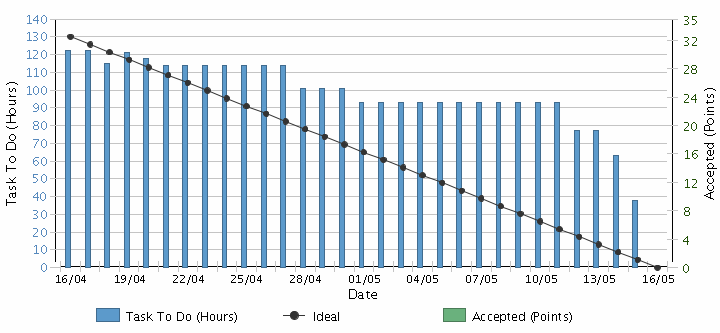
\includegraphics[width=\textwidth]{./imgs/burndown.png}
\end{figure}

\subsection{Product Increment}
\subsubsection{Arquitectura} % (fold)
\label{sub:Arquitectura}

Durante el an\'alisis generamos diversas User Stories de investigaci\'on, estas nos permitieron hacer un an\'alisis de la arquitectura antes de comenzar a implementarla.
Con pruebas de concepto que nos permitieron entender la factibilidad de dicha implementaci\'on.

Los resultados de dicho an\'alisis se encuentra al final de esta secci\'on, en los siguientes parrafos haremos un an\'alisis de la tecnolog\'ia elegida.

\subsubsection{Lenguaje}
La decisi\'on de utilizar un lenguaje de tipado din\'amico fue t\'acita, quisimos evitar las restricciones sem\'anticas que nos impone un lenguaje de tipado est\'atico.  
Tambi\'en buscamos un lenguaje de Objetos Puro, dejando Python afuera de esta decisi\'on.  
Finalmente optamos por Ruby, din\'amicamente tipado, de objetos puro, con closures.


No es casualidad que la elecci\'on del lenguaje nos afectara tambi\'en en la elecci\'on de las tecnolog\'ias de soporte de aplicaci\'on:
\begin{itemize}
    \item Servidor SQL, para el soporte de datos de backend
    \item RESTFul server, para la interfaz de aplicaci\'on
    \item Engine de templating para las vistas
\end{itemize}

\subsubsection{Servidor SQL}
Utilizamos SQLite 3 por su portabilidad y facilidad de instalaci\'on.

\subsubsection{Server}

Para brindar los servicios al usuario, utilizamos HTML con una api HTTPRest. Nuestro servidor es Sinatra. De f\'acil utilizaci\'on solo es necesario conectar los servicios HTTP a la capa del controlador. ¿Por qué decimos que es REST? B\'asicamente no depende del estado, es orientado a cliente-servidor y est\'a orientado en capas.

Esto nos permite desacoplar la aplicaci\'on de la interfaz de usuario, en la versi\'on actual entregamos una interfaz modesta en HAML, un lenguaje de templating cuya transormaci\'on a HTML es nativa en Ruby + Sinatra.

\subsubsection{Modelo}

Para el modelo de aplicaci\'on aplicamos una versi\'on reducida de MVC.

Por un lado tenemos el servidor de aplicaci\'on (sinatra como comentabamos en la secci\'on anterior) y por otro lado tenemos un controller cuyas responsabilidades se ven acotadas a la validaci\'on del input de usuario y la delegaci\'on del procesamiento a ciertas acciones definidas en la capa de servicios.

Los servicios que actualmente soporta el controlador son los de b\'usqueda.

\subsubsection{Extensibilidad}

Nuestro dise\~no como veremos (y justificaremos) en las siguientes secciones, es extensible en:

\begin{itemize}
    \item Tipos de filtros: nuevos tipos de b\'usquedas podr\'an agregarse sin modificar ni la validaci\'on de los par\'ametros ni la interfaz de usuario. Esto lo conseguimos mediante una sencilla t\'ecnica de metaprogramaci\'on.
    \item Tipos de consumo de datos de Twitter: actualmente soportamos la api on-line y la api off-line. 
    \item Estrat\'egias de parsing de twitts: en esta versi\'on acotada utilizamos una extracci\'on de datos posicional por medio de regular expressions, esto podr\'a ser modificado para utilizar un interprete de lenguaje natural que extraiga estos datos cuya ambig\"uedad es tan variada.
    \item Interfaces de usuario: actualmente brindamos una interfaz HTML pero podr\'ia interactuar con una UI distinta, braile, de escritorio, distribuida, etc.
\end{itemize}

% subsection Arquitectura (end)

Principalmente disfrutamos de aprender Ruby, siempre es bueno aprender un lenguaje nuevo.

Creemos que las dificultados no estuvieron en el aprendizaje de nuevas herramientas, si no más bien en tratar de mantener el ritmo de trabajo.

Mención aparte merece el tema del trabajo en equipo. Acá nos encontramos con algunas dificultades, muchas por desconocimiento de cómo trabaja el otro. Ya que salvo Daniel y Hernan el resto nunca había trabajado en un TP juntos. Algunos miembros se adaptaron al dinámica de grupo que se estableció y otros no. 

Esto creemos que afectó en la entrega dado que en la recta final algunos miembros del grupo se sobrecargaron de tareas.

También hicimos mucho foco en las herramientas y la implementación y no tanto en el diseño formal. Nos dejamos llevar por el entusiasmo por lo nuevo, si bien estamos convencidos de que el diseño que pensamos es bueno.

Este foco por la implementación y el ritmo tardío de trabajo hizo que nos comunicáramos poco con el product owner para validar nuestro avance. Tal vez acá nos podría haber llamado un poco más la atención, como entendemos que hubiera sucedido en un escenario real (si bien sabemos que ya estamos grandecitos).

\subsection{Diseño Orientado a Objetos}

\subsubsection{Ciclo de vida de una consulta}

El siguiente diagrama (figura \ref{fig:sequence_sinatra}) muestra la interacción en los distintos componentes de la aplicaciones. Los distintos componentes serán explicados en las sucesivas secciones.

\begin{figure}[h]
\centerline{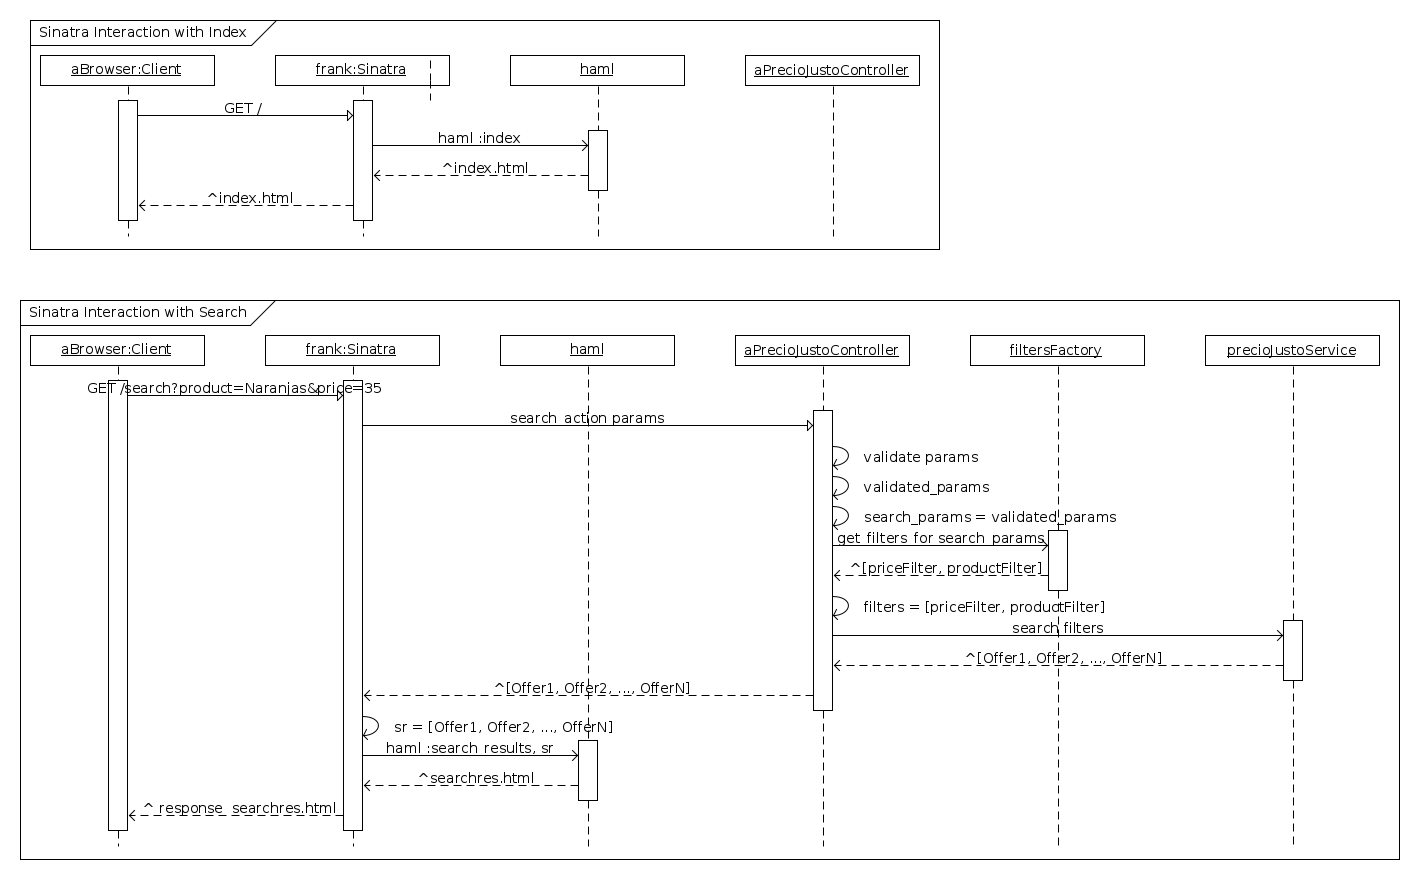
\includegraphics[width=0.9\paperwidth]{./imgs/sequence_diagram_sinatra.png}}
\caption{Diagrama de secuencia de sinatra}
\label{fig:sequence_sinatra}
\end{figure}


\subsubsection{Factory de servicios}
Dado que twitter permite dos tipos de obtención de tweets, vía streaming o por búsquedas, es que implementamos dos formas de trabajar con los tweets, pero que desde el lado de clientes de la búqueda de ofertas de El Precio de Justo mantienen la misma interfaz.

Para esto último decidimos utlizar el patrón de \texttt{abstract factory} con dos
implementaciones, una online y otra offline. Cada una de estas implementaciones nos permiten crear la clase de servicio apropiada (la clase que encapsula la lógica de la aplicación), los filtros permitidos y la implementación específica de estos.

Esto puede verse en la figura \ref{fig:class_service_factory}.

\begin{figure}[h]
\centerline{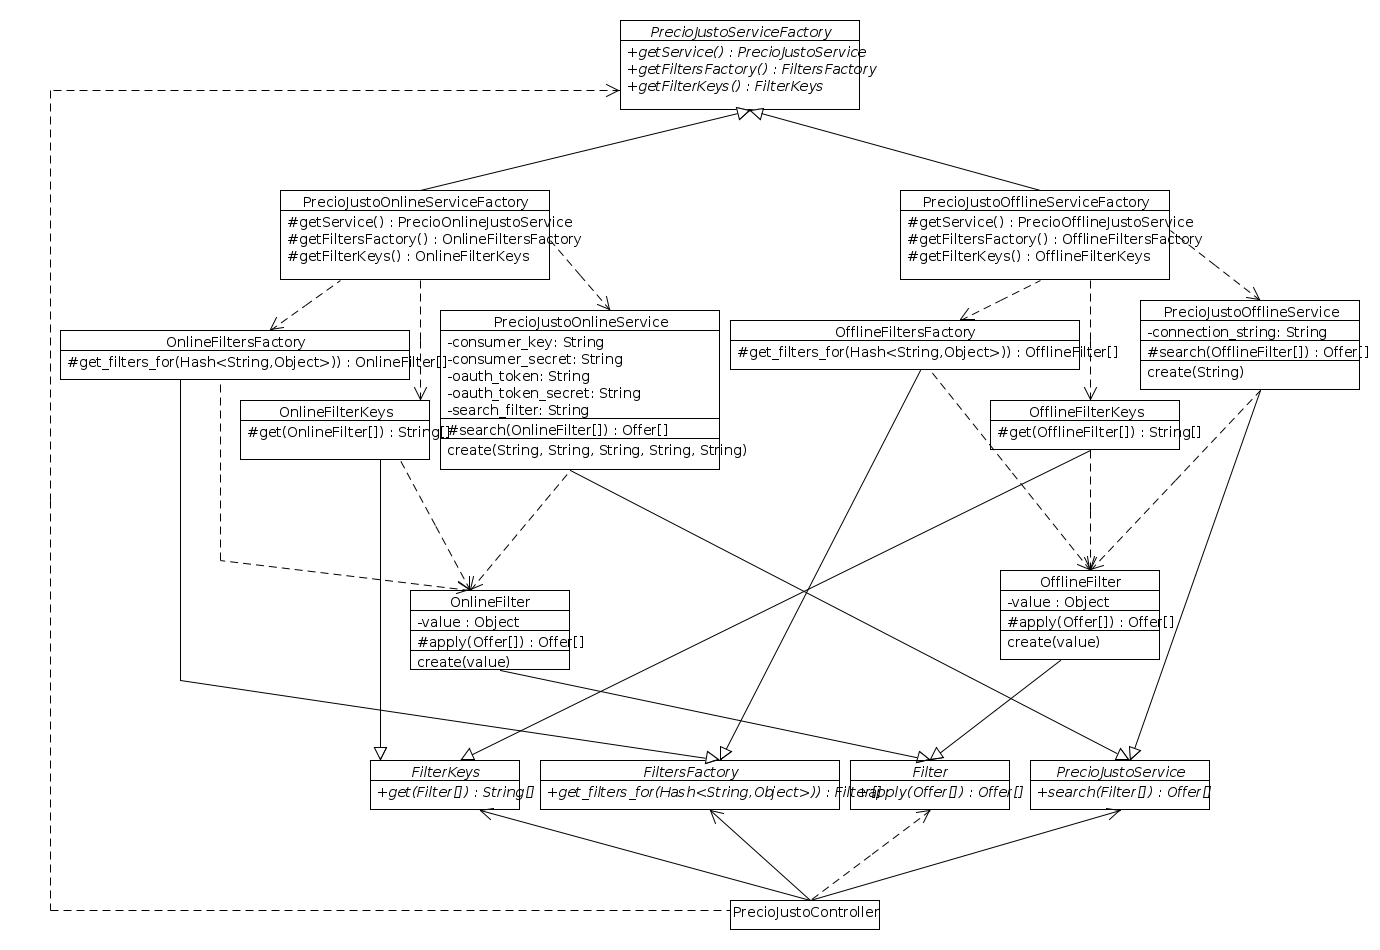
\includegraphics[width=0.9\paperwidth]{./imgs/class_diagram_service_factory_v2.png}}
\caption{Diagrama de clases de creación de servicios}
\label{fig:class_service_factory} 
\end{figure}

\subsubsection{Filtros}

Dado que el filtrado de los tweets de las ofertas búscadas se realizan de distinta manera, los filtros si bien deberán proveer las misma funcionalidad son implementativamente distintos.

En un caso filtrarán las ofertas que se vayan obtienendo de twitter en vivo y en el otro caso se realizará un búsqueda sobre el motor de base de datos.

Los filtros modelados son por porducto, precio y ubicación, si bien es posible extenderlos.

Esto puede verse en el diagrama de la figura \ref{fig:class_filter_factory}. 

\begin{figure}[h]
\centerline{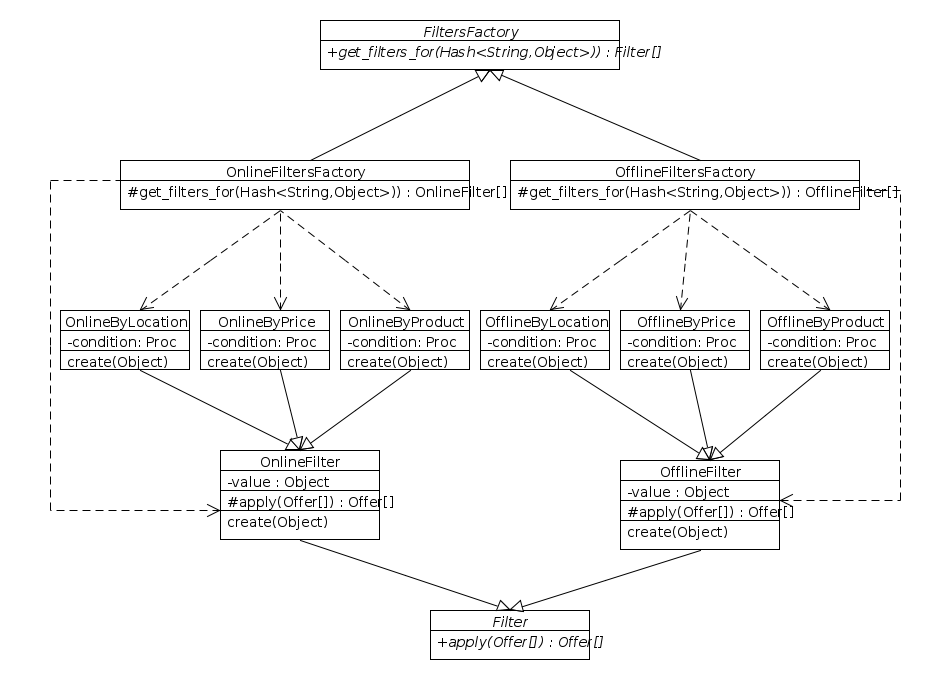
\includegraphics[width=\textwidth]{./imgs/class_diagram_filters_factory.png}}
\caption{Diagrama de clases de creación de filtros}
\label{fig:class_filter_factory} 
\end{figure}

\subsubsection{Extracción de datos de un tweet}
La extracción de las información de las ofertas que se encuentra en los tweets se realizar mediante objetos de la clase \texttt{OfferFromTweetExtractor} (clase abstracta).
Para la demostración realizamos una implementación que extrae la información mediante expresiones regulares para cada pedazo de información dentro del texto, salvo para la geolocalización del tweet.
Si bien no está implementado para la demo, es deseable delegar la creación de las instancias de Offer. Para ello pensamos realizar mediante un \texttt{OfferBuilder}, la tarea del mismo sería realizar las acciones necesarias para crear una nueva instanacia.

La idea es que cada pedazo de información genere una instancia de un objeto polimórfico de la información que modela (ej: el precio, producto, unidad).
Cuando nos referímos a objetos polimórficos, queremos decir que la información podría no poder generar un objeto válido y queremos que resulte transparente para los objetos con los que interactuan con dicho objeto (la idea es poder implementar \texttt{Null Object Pattern})

\begin{figure}[h]
\centerline{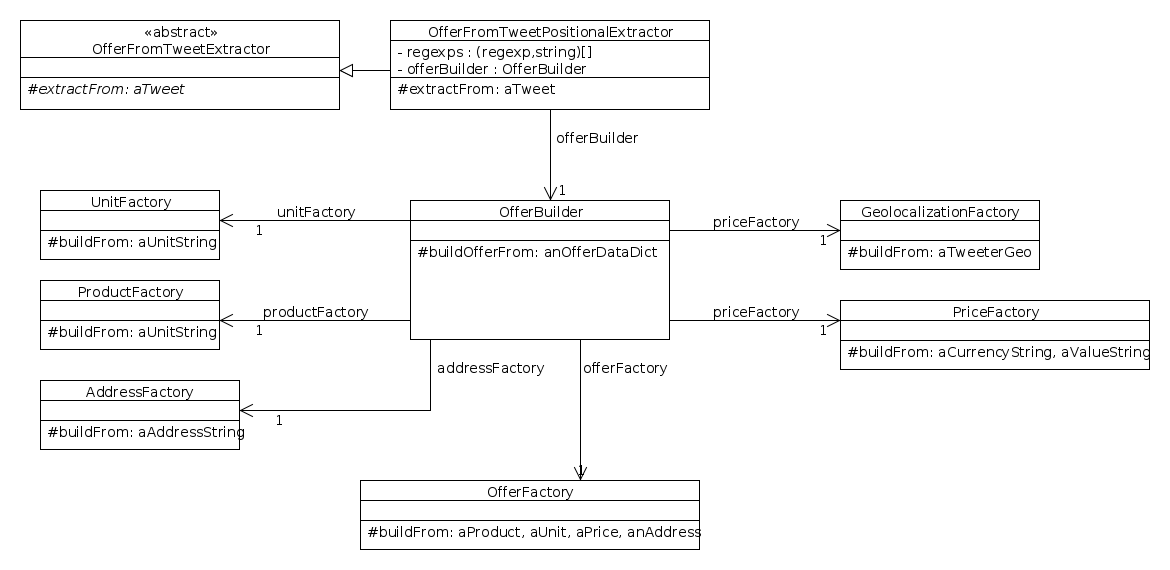
\includegraphics[width=\textwidth]{./imgs/class_diagram_parsing.png}}
\caption{Diagrama de clases de extraccion datos de tweet}
\label{fig:class_parsing}
\end{figure}

\begin{figure}[h]
\centerline{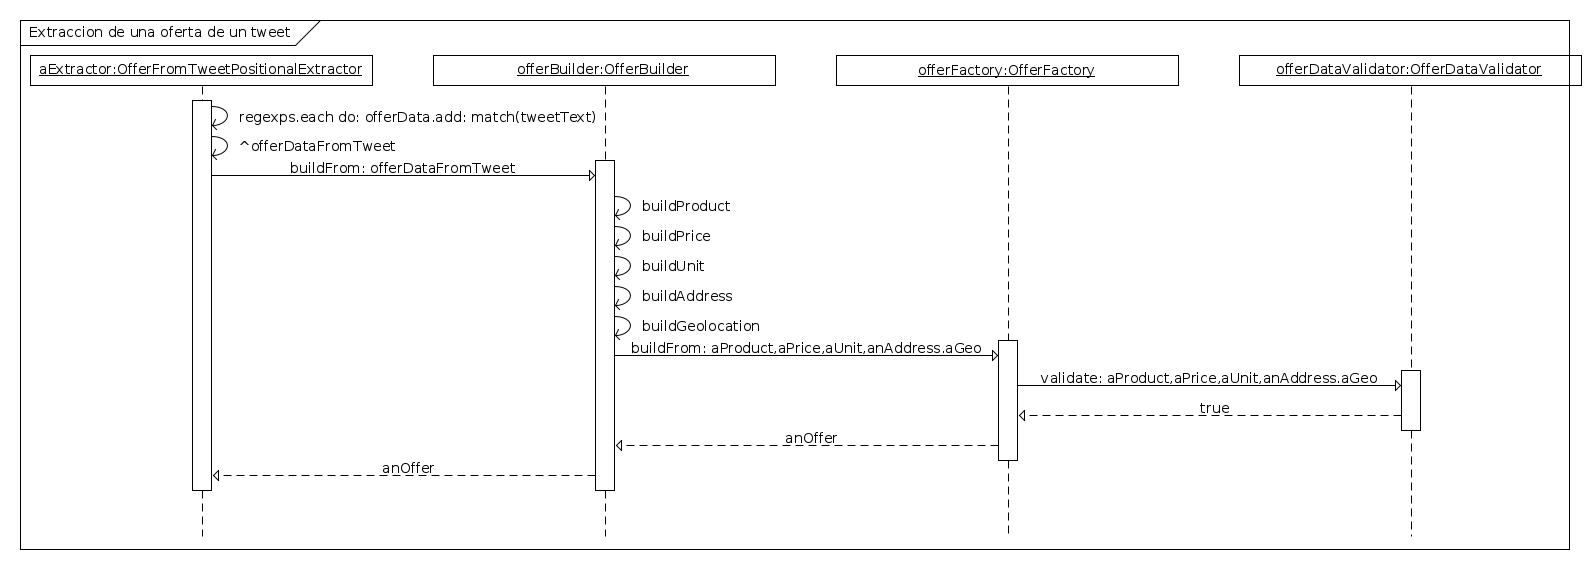
\includegraphics[width=\textwidth]{./imgs/sequence_diagram_parsing.png}}
\caption{Diagrama de secuencia de extraccion de datos de tweet}
\label{fig:secuence_parsing}
\end{figure}

\subsubsection{Servicio Online}
En este caso la clase PrecioJustoOnlineService encapsula la lógica de la aplicación utilizando como fuente de información las búsquedas directas en \texttt{Twitter} mediante la \texttt{API} de \texttt{Search}.
Para aplicar los filtros utiliza las clases derivadas de \texttt{OnlineFilter} y utiliza \texttt{OfferFromTweetPositionalExtractor} para la extracción de las ofertas.

\begin{figure}[h]
\centerline{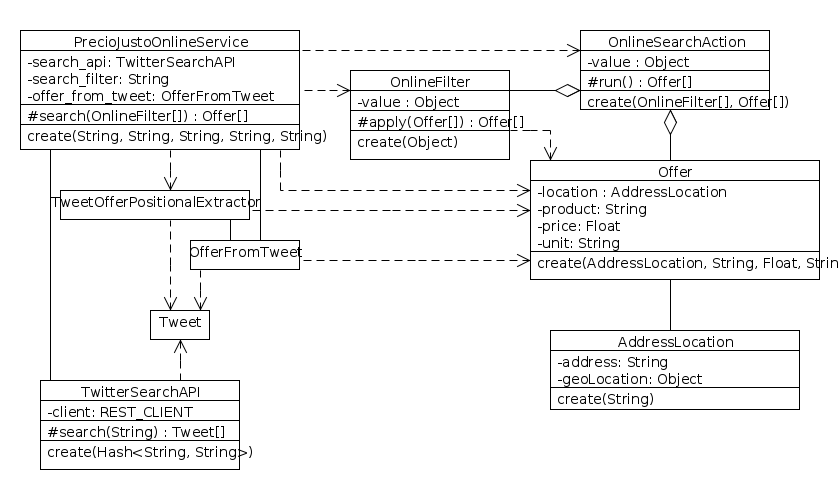
\includegraphics[width=\textwidth]{./imgs/class_diagram_online_service.png}}
\caption{Diagrama de clases de servicio online}
\label{fig:class_online_service}
\end{figure}

\subsubsection{Servicio Offline}

\textbf{PrecioJustoOfflineService}\\

En este caso la clase \texttt{PrecioJustoOfflineService} encapsula la lógica de la aplicación utilizando como fuente de información una base de datos \texttt{SQLite3}. La cual es alimentada mediante un servicio independiente.
Para aplicar los filtros utiliza las clases derivadas de \texttt{OfflineFilter}. Las ofertas
ya fueron parseadas antes de ser insertadas en la base de datos.

\begin{figure}[h]
\centerline{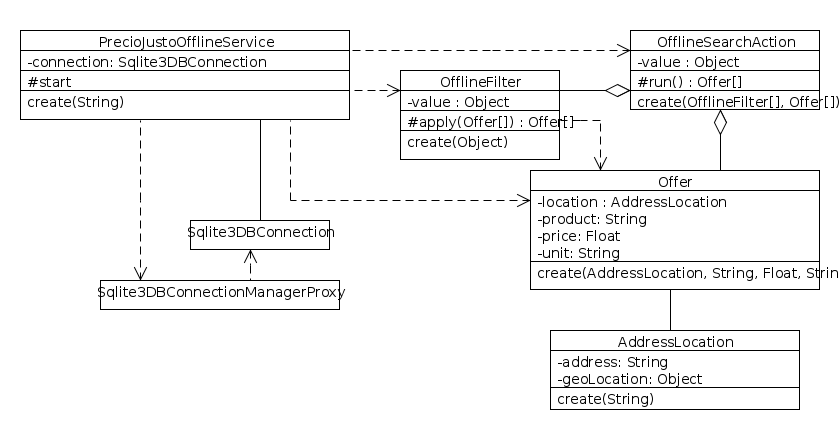
\includegraphics[width=\textwidth]{./imgs/class_diagram_offline_service.png}}
\caption{Diagrama de clases de servicio offline}
\label{fig:class_offline_service}
\end{figure}

\textbf{Servicio de Streaming}\\

Este proceso independiente utiliza la \texttt{API} de \texttt{Streaming} de \texttt{Twitter} para obtener las ofertas y persistirlas en la base de datos.
Para la extracción de las ofertas de los tweets utiliza el extractor \texttt{OfferFromTweetPositionalExtractor}.

\begin{figure}[h]
\centerline{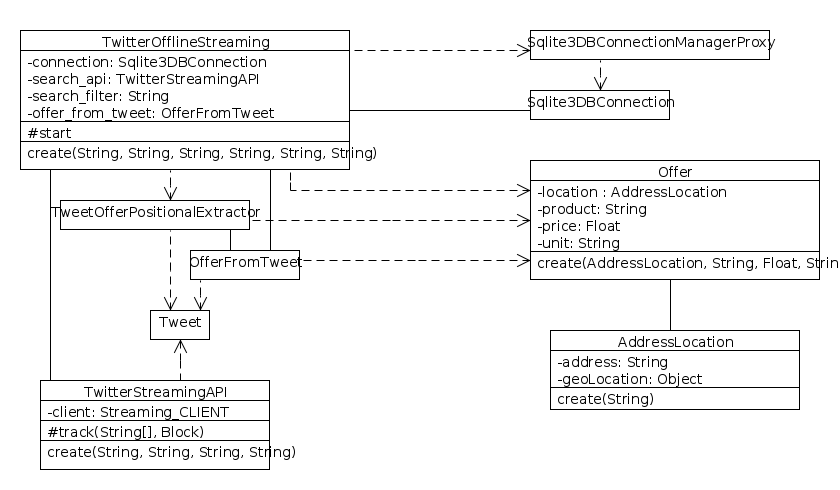
\includegraphics[width=\textwidth]{./imgs/class_diagram_offline_streaming.png}}
\caption{Diagrama de clases de streaming de twitter}
\label{fig:class_offline_streaming}
\end{figure}


\textbf{Cliente/Servidor SQLite3}\\

Dado la base de datos \texttt{SQLite3} es un archivo, el mismo se bloquea al accederlo
directamente. Para evitar esto generamos un proceso independiente que es el único que bloque el archivo, pero expone mediante \texttt{DRB (remoting)} la conexión a esta base para poder ser usada concurrentemente por distintos proceso.

\begin{figure}[h]
\centerline{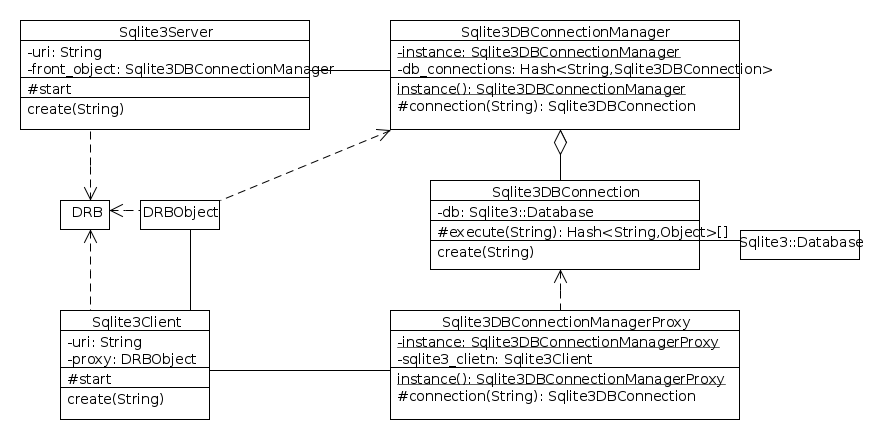
\includegraphics[width=\textwidth]{./imgs/class_diagram_sqlite3_client_server.png}}
\caption{Diagrama de clases de BD SQLite3}
\label{fig:class_sqlite3_client_server}
\end{figure}

\textbf{Ofertas y colaboradores}

El siguiente diagramas muestra el modelo de las ofertas (\texttt{Offer}) y sus colaboradores. Dichos colaboradores no están modelados en la demostración.
El siguiente diagramas muestra la idea de creación de los distintos objetos
con la idea de poder generar objetos no válidos polimórficos a los válidos.

\begin{figure}[h]
\centerline{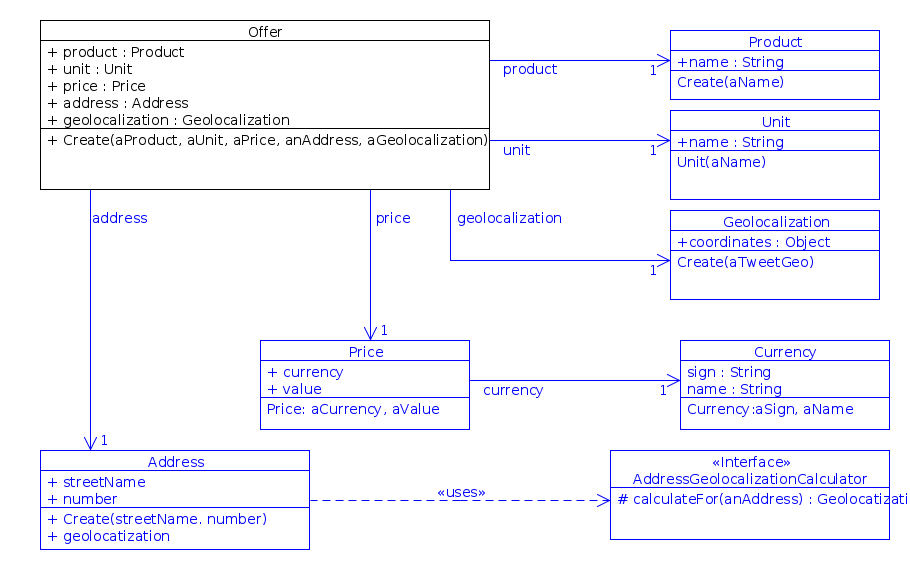
\includegraphics[width=\textwidth]{./imgs/class_diagram_offer.png}}
\caption{Diagrama de clases de offer y colaboradores}
\label{fig:class_offer}
\end{figure}

\begin{figure}[h]
\centerline{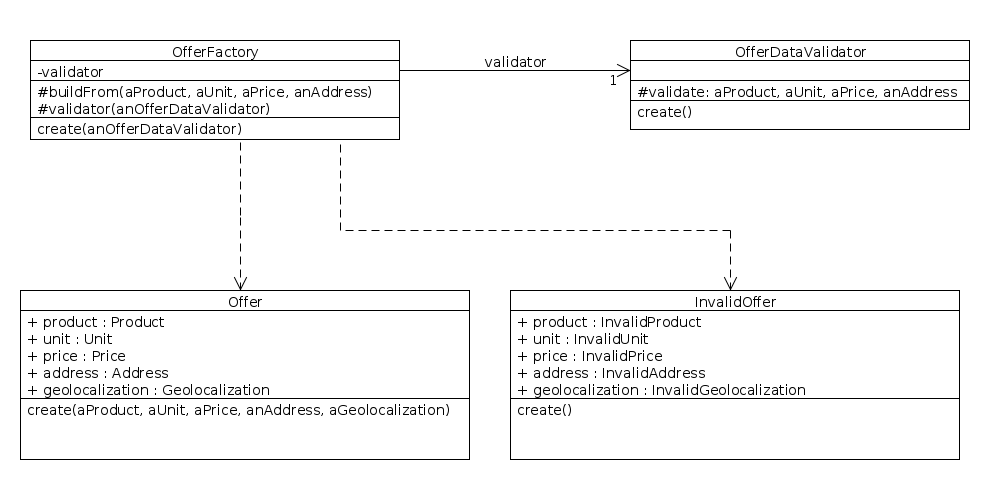
\includegraphics[width=\textwidth]{./imgs/class_diagram_Offer_Factory.png}}
\caption{Diagrama de clases de creación de offer}
\label{fig:class_Offer_Factory}
\end{figure}




\end{document}
